\chapter{\Tigrisd: 一个轻量定理证明器}
\renewottcommands[dd]

\Tigrisd 是一个试验性质、以依赖类型作为理论基础的定理证明器。\Tigris 与 \Tigrisd 一同，
构成了一套 PL(DI)/定理证明教育解决方案。\Tigrisd 在设计与实现上，
受到了 Lean、pi-forall、LambdaPi、elaboration-zoo 项目的深刻影响。

目前而言，\Tigrisd 使用 Haskell 实现，因其强壮、活跃的生态环境，拥有诸如 \texttt{Unbound} 等用于
操作\lambdacalc、AST 的库使得我们不必重新造轮子\footnote{
  相较而言，\Tigris 就是一个（几乎）全数独立实现的子系统。
  其中用到的许多函数、实现都是针对这一语言特化的，因而较难将之迁移到此处为 \Tigrisd 所用。
}。
虽然我们未来展望有一天能将之用 Lean 重写，并配套一个定理证明过（verified）的实现——重点是
当下已经拥有一个可以工作的原型。

在实现上，\Tigrisd 只包含四大部分：句法分析器、内核、命令行前端。
这一部分主要介绍内核的设计与实现，并提供一个简单的范例展示证明。

\paragraph{命名规范} “项（term）”一词，当单独使用时，包含常规语言（非依赖类型）中的\emph{类型}。
当“项”与“类型”一起使用时，大部分情况下前者不包括后者。“类型”永远指代类型，无论依赖与否。
“内核”一词可看作类型检查器的同义词。

\section{语言基础与基本概念}
\Tigrisd 所支持的语法与 \Tigris 极为相似，仅有少数例外，且都与前者作为依赖类型语言相关。
这一语法的实现仍然使用基于组合子的单子句法分析，其特殊之处在于 \emph{layout} 组合子，这一组合子
使用 off-side rules（缩进影响语义，如 Haskell）。这一例外是因为证明通常比程序更复杂，一些语法中的
连接词，如 \texttt{let..in} 中的 \texttt{in}，在依赖缩进的语法中可以省略，降低\emph{语法噪音}，
提升可读性。下面叙述重要语法构造的区别。

\paragraph{枚举族} 是前述代数数据类型的“升级版”。
\begin{definition}[枚举族声明] 由以下 BNF 给出
\begin{minted}{bnf}
<dtype-decl>    ::= inductive <dtype-name> <dtype-ibinder>* : Type
                    "where"? ("|" <dtype-branch>)*
<dtype-branch>  ::= <dtype-ctor> : sepBy1("->", <dtype-binder>)
<dtype-ctor>    ::= <upper-ident>
<dtype-name>    ::= <upper-ident>
<dtype-binder>  ::= <dtype-tbinder> | <dtype-ibinder>
<dtype-tbinder> ::= (<ident> : <term>)
<dtype-ibinder> ::= {<ident> : <term>}
\end{minted}
\end{definition}
例如一个将长度\emph{嵌入}类型的列表（换句话说，类型依赖长度）可定义为：
\begin{minted}[frame=single]{lean4}
inductive Vector (α : Type) (n : Nat) : Type where
  | Nil                                      where n = Zero
  | Cons {m : Nat} (x : α) (xs : Vector α m) where n = Succ m
\end{minted}
其中我们使用花括号 \texttt{\{\}} 表示类型无关（不参与编程计算）的绑定子。
构造子的结果类型将与定义类型做比较，确保两者的\emph{头}一致，在此处即 \texttt{Vector}.
这一声明显式地规定了两条约束，按分支分别为 $n = 0$ 与 $n = \mathsf{Succ}\ m$. 通过 \texttt{example} 关键字，
我们能引入匿名的定义用于测试这个类型的可用性：
\begin{minted}[frame=single]{lean4}
example: {α : Type} -> Vector α 0 := Nil
example: Vector Unit 2 := Cons 1 () (Cons 0 () Nil)
\end{minted}
\paragraph{函数} 定义现在有形式
\begin{definition}[函数定义] 由以下 BNF 给出
\begin{minted}{bnf}
<tm-lam>      ::= fun <dtype-binder>+ => <tm>
<tm-toplevel> ::= def <ident> <dtype-binder>* : <tm> := <tm>
\end{minted}
\end{definition}
注意：\Tigris 中介绍的 pattern matching let 语法糖并不适用于此处。若想使用模式匹配，
必须通过 \mintinline{lean4}|fun pat => ...| 语法糖或以下最基本形式使用：
\begin{minted}[frame=single]{lean4}
def map {α β : Type} {n : Nat} (f : α -> β) (as : Vector α n)
  : Vector β n :=
  match as with
  | Nil         => Nil
  | Cons m x xs => Cons m (f x) (map {α} {β} {n} f xs)
\end{minted}

\Tigrisd 目前并不具备隐式变量推断（implicit inference）或隐式项合成（implicit synthesis），因而我们
要求用户提供所有绑定的参数，如上例所示。\Tigrisd 的类型检查器仅实现一简单的双向算法，只具备有限的
推断能力。
应当铭记下述 \Tigris 与 \Tigrisd 在函数定义上的差距，暨依赖类型论最显然的特征，
\begin{center}
  \underline{函数能接收\emph{类型}作为参数，就像其能接收值一样，因为\emph{类型也是项}}。
\end{center}
这一特性产生了一些在 \Tigris 中需要拓展类型系统（例如 skolems）才能实现的规则。考虑将第二个分支的右手侧递归应用 \texttt{map xs ..} 替换成
\texttt{xs}，使得整个式子成为 \texttt{Cons m (f x) xs}——检查器将立马报错，因为其需要证明 $\mathsf{Vector}\ \alpha\ n$、$\mathsf{Vector}\ \beta\ n$
相等，即证 $h : \alpha=\beta$.\footnote{
  依赖类型论的\emph{相等性}是一个极为重要的概念，我们将在下一节给出具体介绍。
}显然根据现有信息，不可能证出上述等式，因为等号两侧是随机选取的类型。

\paragraph{模式匹配与（依赖类型）元组消去} 已经被减少到以下两种语法形式：
\vspace{-.8em}
\begin{itemize}\itemsep-.5em
    \item \mintinline{lean4}|match e with ..| 只接受构造值模式；
    \item \mintinline{ocaml}|let (x, y) := a in b| 并非上述结构的语法糖，而是用于实现
    （依赖类型）元组消去的语法构造。
\end{itemize}
\vspace{-.8em}
关于上一部分提到过的 discriminant refinement，\Tigrisd 亦支持，我们将在后文介绍。

\paragraph{类型/证明无关性} 指的是类型、证明一定被擦除而不出现在最终的程序中的性质，因为
两者并没有运行时表示。显然，对于类型检查器来说，确保擦除正确，不意外擦除\emph{有意义的}值十分重要。
\emph{无关性}（irrelevance）一词指上述现象，但并非只有证明和类型是无关的，在下文我们还能看到其他的无关项。

\paragraph{模块} 与 \Tigris 一致。任一 \Tigrisd 源文件自动构成一模块，由源文件名作为模块名。此外，
我们也实现了类 Haskell 文件顶端的声明：通过 \mintinline{haskell}|module X where| 定义一个模块 $X$,
由顶端声明 \mintinline{lean4}|import M1,..,M2| 将 $M_1,\dots,M_i$ 引入当前模块。

\paragraph{内置证明} 是 \Tigrisd 内建的证明手段。共五种，前四种为原生构造，后一种为语法糖。

\texttt{sorry}（证明）：可用于证明任意命题，显然是不合理的。实际使用中，我们用此
来标记一个未完成的证明，方便之后补全，而不使得编译器报错。此命令的任一使用都会触发编译器的报警，
并使得其本身和与之相关的所有定义都被标记为\emph{不相关}。

\texttt{rfl}（证明）：为 reflexivity（自反性）的简写，可证明 $a = a$，对任意项 $a$. 可以说这是
所有等式命题的\emph{根证明}，因为更复杂的证明无非是将等式的任一一侧变换成另一侧，并通过自反性得证。\texttt{rfl}
远比其看起来的复杂：其支持 $\alpha$-等价 和 $\beta$-等价，即经过任意有限步 $\alpha$/$\beta$-变换的两个项
在 \texttt{rfl} 下直接相等。

\texttt{exfalso tm}（证明）：即爆炸原理。\texttt{exfalso} 接收一个证伪的项，
以此证明任意命题，或“构造”任意类型的一个值。在没有假设的前提下，若独立证出证伪的项，说明
系统不合理（unsound）。

\texttt{(|>)}（证明）：即等式重写。表达式 $h\triangleright e$ 在左手侧接受一等号类型 $a = b$ 的证明 $h$，
在右手侧要求 $e = a$，则可以证明 $b$.

\texttt{nomatch tm}（证明）：表示模式匹配 $tm$ 不存在任何分支，可以看作是另一种形态的爆炸原理。
给定空类型 \mintinline{lean4}|inductive Empty|，若 \Tigrisd 能证明其不含任何 introduction rule（构造子），
则模式匹配其值 $tm$ 时可用 \texttt{nomatch} 证明任意命题，如
\begin{minted}[frame=single]{lean4}
example (h : Empty) (C : Type) : C := nomatch h
\end{minted}
在实现上，这些命令基本被硬编码到核心代数 \mintinline{haskell}|Term| 中，且有定义

\begin{minted}[numbers=left]{haskell}
type Type = Term
data Term = Type0 {- 非直谓的类型宇宙 -} | {- .. 略 .. -}
  | Sorry {- sorry 证明 -} | Print {- show 命令 -} | Rfl {- rfl 证明 -}
  | Rw Term Term {- (|>) 证明 -} | Contra Term {- exfalso 证明 -}
\end{minted}
其中，我们还定义了别名 \mintinline{haskell}|Type| 并将之绑定到项（\mintinline{haskell}|Term|）上：从这里
也可看出依赖类型论的特点：类型也是项。此外，上面提到的 \texttt{nomatch tm} 证明则并非由硬编码得到，
而是在句法分析阶段直接解糖成为模式匹配 \mintinline{ocaml}|match tm with|，但其不含任何分支。

搭配 \texttt{Unbound} 库，可以轻松的为这一核心代数实现 \lambdacalc 中最为重要的两个操作：\emph{$\alpha$-相等}判断
与\emph{变量代换}。

\begin{Verbatim}[numbers=left,baselinestretch=1]
instance Unbound.Alpha Term where
  aeq' ctx a b = gaeq (strip a) (strip b) where
    gaeq = Unbound.gaeq ctx `on` from
instance Unbound.Subst Term Term where
  isvar (Var x) = Just (Unbound.SubstName x)
  isvar _       = Nothing
\end{Verbatim}

其中 \texttt{aeq} 即 $\alpha$-相等，\texttt{isvar} 则用于判断核心代数中哪些是可以用于代换的变量；\texttt{on} 中缀应用
可以看作是二元函数的复合算符。给定函数 $f : \beta\to\beta\to\beta,\, g:\alpha\to\beta$，$f\ \mathrm{on}\ g:\alpha\to\alpha\to\beta$ 是
$f$ 在 $g$ 上的投影。

\paragraph{类型宇宙} 亦称 level，在 \Tigrisd 中只有一个，且是\emph{非直谓的}，即 \mintinline{lean4}|Type : Type|，而非 \mintinline{lean4}{Type 1}，读作类型宇宙 \mintinline{lean4}{Type}，存在于自身中，或
\mintinline{lean4}{Type} 的类型还是 \mintinline{lean4}|Type|. 虽然单一宇宙的直觉类型论
（Martin-Löf/Intuitionistic Type Theory，MLTT. 依赖类型论的一种，但也可作为其别称）已由
Girard 证明不合理\footnote{
  我们并不细究其为何不合理，因为那是数学家的工作。读者只需知道其原因类似为什么 ZF 集合论中需要
  正则公理；否则会产生罗素式（Russell-style）的悖论。
}，我们仍然以之作为理论基础，因其简单性。此外，有界递归、停机/完备性检查在 \Tigrisd 中都不存在。

\section{\Tigrisd 内核的形式化描述与实现细节}
类似第二部分，下面我们给出 \Tigrisd 内核的形式化描述，但同时在每一要点中附带实现介绍。
由于类型亦属于项，所以我们不再区分类型系统和值，统归于核心代数下。
\allowdisplaybreaks
\paragraph{核心代数与类型环境} 由于篇幅所限，我们略过核心代数的叙述，读者应当能够直接从
下方的判断规则中得知。首先给出类型环境上的操作，

%\nonterms[0pt]{tm}
%\nonterms{context}

\drules[g]{$\Gamma$}{Context construction}{nil, cons}
项的类型判断规则为
\drules[t]{$\Gamma\vdash a : A$}{Typing}
{ var
  , refl
  , impred-univ
  , app
  , cast
  , pair
  , eq
  , exfalso
  , lambda
  , pi
  , sigma
  , letpair
  , let
  , subst
, exfalso}

其中 $\Pi/\Sigma$ 类型分别表示依赖积/余积（dependent product/coproduct）类型。
Product，如其形式，与箭头类型 $(\cdot\to\cdot)$ 极为相似，可以看作其“升级版”。
区别在于，现在我们为箭头左手侧（逆变位置）
增加了一个标识符（label），允许箭头右侧提及左侧，即结果类型依赖于参数。显然，依赖积可以用于编码
函数类型，且如果出现在类型层面，可以用于编码 $\forall$ binder ——依赖类型论“免费给予”我们一般语言
中的参数多态，且毫不费力。
同理，coproduct 的右手侧也可
依赖左手侧，可用于编码元组类型。这两个类型的叫法很多，例如前者亦称 dependent function type，后者
称 dependent sum type. 为了表述清晰，我们统一使用范畴论术语 product/coproduct.

我们略去一些常量（$\mathsf{Bool}$、$\mathsf{Unit}$）的规则，因为这些规则
与 \Tigris 一致。不相关项的类型规则同上，但另外给出：

\drules[t]{$\Gamma\vdash a : A$}{Irrelevant Typing}{elambda, eapp, epi}

\Tigrisd 的双向类型算法存在两个类型判断（judgement）：检查与推断。这两个判断在实现中对应两个
（互）递归的函数 \texttt{infer}、\texttt{check}. 显然，两者是互相依赖对方的。此外，对于
类型检查器来说，上述两个判断其实是两个\emph{模式}，对于不同的语法结构，我们采用不同的模式：
例如当其遇到 \rref{C-lambda} 时，是检查模式；遇到 \rref{I-app-nonwhnf} 时，是推断模式。
这两个模式分别用类型判断 $\Gamma\vdash a\Leftarrow A$、$\Gamma\vdash a\Rightarrow A$ 表示。显然，
如果这个系统是\emph{正确}的，则应当满足
{\setlength{\abovedisplayskip}{3pt}\setlength{\belowdisplayskip}{3pt}
  \begin{align*}
    \Gamma\vdash a : A\ \text{if}\ \Gamma\vdash a\Leftarrow (A : \mathbf{Type})\wedge
    \Gamma\vdash a : A\ \text{if}\ \Gamma\vdash a\Rightarrow A
  \end{align*}
}
汇总起来，我们针对两个模式给出对应的类型规则。
\drules[c]{$\Gamma\vdash a\Leftarrow A$}{type checking}
{ lambda
  , refl
  , pair
  , switch-mode
  ,exfalso, let
  , letpair-RL
  , letpair-LR
  , subst-l
  , subst-r
}
\drules[i]{$\Gamma\vdash a\Rightarrow A$}{type inference}
{ var
  , app-nonwhnf
  , impred-univ
  , pi
  , ascribe
  , sigma
  , let
  , eq
  , app
, subst}

\paragraph{相等性} 一些读者可能注意到上述推断规则中出现了定义性相等\footnote{
  在 MLTT 中也是判断性（类型规则见下文）相等；在单一宇宙 TT 中是类型上的相等。
}，例如 \rref{C-switch-mode, I-App}. 这是因为在类型作为项的类型检查中，
若要确认两个类型（变量）相等，可能需展开其定义并做一些计算才能确定——不妨先解决\emph{什么是相等}这一问题。

在各种类型论中，有诸多不同但又相关（甚至交叉）的
相等性（equalities），例如元相等（meta\textasciitilde）、定义性相等（definitional\textasciitilde）、判断性相等（judgemental\textasciitilde）、命题性相等（propositional\textasciitilde）、类型上的相等（typal\textasciitilde）。
这些相等性的区别与交叉体现了不同类型论建模“相等”这一概念的不同思路。下文主要介绍 \Tigrisd 的类型论涉及的前三个概念。

\subparagraph{元相等}指那些非内化于类型论的相等性。之所以称其“元”，是表示其存在于类型论之上（不是在
类型论中定义的），定义在\emph{元理论}（可理解为实现）中的特点。最明显的例子是，若两个项具有相同
\emph{形状}——AST 相等（syntactic equality，语法上相等）——则它们\emph{一定相等}，
\underline{无论类型论如何}——\emph{语法相等}就是元相等的一种，所有类型论都具备这一相等性。
同时，绝大多数类型论都以\lambdacalc 作为核心代数，因此元相等性也包括 \emph{$\alpha$-等价}\footnote{
  $\alpha$-equivalence 指出，形式语言中的两个式子（例如类型、项、命题、环境等）等价，若它们仅存在
  \underline{约束（绑定）变量名字上的不同}。
}。
在 \Tigrisd 中，
元相等恰为此二种，其中后者通过 \texttt{Unbound} 库实现。该库提供了用于替换、计算自由变量、生成崭新变量
等一系列\lambdacalc 上的操作，避免重新造轮子带来的不便，也使我们的实现经得起考验。
例如上述包含 $\alpha$-等价的元相等、自由变量的计算，在 \texttt{Unbound} 库中即为函数
\begin{minted}[numbers=left]{haskell}
aeq :: Alpha a => a -> a -> Bool -- 中缀算符 '==='
fv  :: ( Alpha a, Typeable b
       , Contravariant f, Applicative f) => (Name b -> f (Name b)) -> a -> f a
id x = Lam $ Unbound.bind x $ Var x -- 在源代码中构建一个 Tigrisd 中的恒等函数的 AST
id 'x' === id 'y' -- alpha-equiv: (\x -> x) === (\y -> y): >>> True.
\end{minted}
\subparagraph{定义性相等}可以看作元相等的“升级版”。
准确地说，定义性相等是定义在\emph{式子}上的\emph{等价关系}（注意：并非\emph{等于}关系！），
它指出两个式子是等价的，若其具有相同的\emph{含义}——显然，它蕴含元相等。

定义性相等是\emph{内涵的}（intensional），与另一逻辑概念\emph{外延}相对。
前者关注的重点在于某一对象的具体\emph{定义}，后者在于该对象的\emph{外在表现}，或\emph{行为}。以集合为例，
“小于 3 的正整数集”是一集合的\emph{内涵定义}，而 $\{1,2\}$ 是其唯一的\emph{外延表述}。
在类型论上，具有相同意义的式子是\emph{内涵相等}的。

之所以称其为“升级版”，是因为绝大多数类型论都会在其\emph{理论内}再定义\emph{显式定义性相等}，后者与元相等统称\emph{定义性相等}。
重点在于，\underline{这些理论是\emph{如何}在其内部定义上述等号的}——由此引伸出三种类型论上的等号：判断性相等、命题性相等、类型上的相等。需要注意的是，三种等号并不一定互斥，例如 \Tigrisd 就满足其中不止一种的等号。
读者不妨与 \Tigris 的类型系统作比较：为什么我们不谈它的相等性呢？显然，
这是因为传统语言的类型系统允许的类型过于简单，
或者说，任何非依赖类型论中存在的项（类型）都过于简单，仅靠元相等，即类型 AST 上的比较便可实现。

此外，\emph{元相等}是所有类型论具有的共性。为做区分，定义性相等一词有时特指显式定义性相等。

\subparagraph{判断性相等}是类型论中最基础的等号。正如其意，判断性相等是在类型论中直接作为
一条判断规则引入的，比如后文将介绍的 $\Gamma\vdash A = B$——\Tigrisd 类型论的等号就是判断性相等。
通常（也包括 \Tigrisd）这一等号就是常规意义上的等于，满足自反性、交换性、传递性——将满足这些性质的
判断性相等称为\emph{判断性等价}。

判断性相等虽然基本，但不代表其使用广泛。主流定理证明器，特别是以 CIC 作为理论基础的，例如 Lean，使用
命题相等性。

\subparagraph{命题相等}适用于两层（即区分类型和命题的）类型论。这一表述与 Curry-Howard 同构的“命题即类型”
表述不冲突：以 Lean 为例，所有的命题存在于类型宇宙（此处称命题宇宙）$\mathbf{Prop}$ 中，所有的类型存在于 $\mathbf{Type}\ u/\mathbf{Sort}\ (u+1)$（其中 $u$ 是宇宙层级）\footnote{
  满足 $\mathbf{Type}\ u\equiv\mathbf{Sort}\ (u+1)$，$\mathbf{Sort}\ 0\equiv \mathbf{Prop}$，
  $\mathbf{Sort}\ 1\equiv \mathbf{Type}$.
}
中。命题仍然是类型，但其基底集为 Subsingleton（次单元素集合），即含有\emph{最多 1 个}
元素的集合。在这一情况下，等式 $1 = 0$ 实际上是（命题）类型 $\mathsf{Eq}\ 1\ 0$，故而
称其命题相等：由命题编码的等号。之所以这样处理，原因是多方面的，但最显著的原因之一即是方便命题无关性的实现。

\subparagraph{类型上的相等}与命题相等类似：由类型编码的等号，例如 Cubical TT、HoTT（同伦类型论，homotopy\textasciitilde）
\footnote{
  虽然后者采用的是“命题为类型”（proposition as types）的解读，应当算作命题相等。
}抑或任意基于\emph{泛等公理}（univalent axiom）的类型论的路径等号。一般把这个
类型称为恒等类型（identity type）或相等类型（equality\textasciitilde），记作 $\mathsf{Id}_A(x, x')$，对
某 $(x, x' : A\times A)$. 由于恒等类型自身在不同类型论中具有不同表述，且其性质涉及到同伦理论、范畴和拓扑
理论的知识，如图 \ref{fig:id-intro}，超出本文范围，我们在此不表。
\begin{figure}\centering
  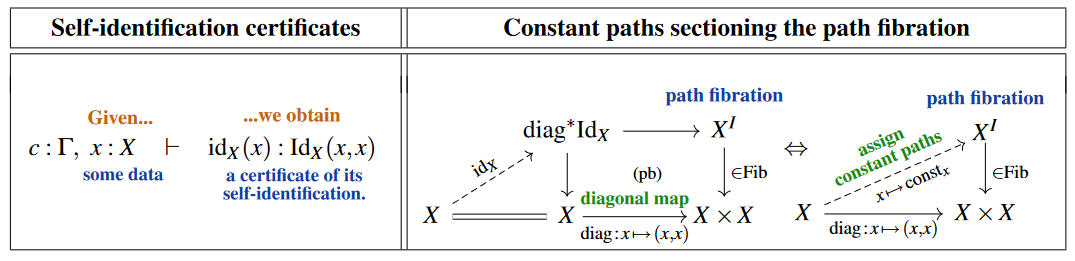
\includegraphics[scale=.9]{assets/MetaLogicOfIdentifications-1-220927.png}
  \caption{恒等类型的引入规则（introduction rule）在范畴论上的意义}\label{fig:id-intro}
\end{figure}

除此之外，类型上的相等在单一层级类型论中亦常见，根据 \rref{T-EQ} 可知，在 \Tigrisd 中，等号也是类型；同时，
我们摒弃恒等类型的记号，仍用等号，以强调其“相等”性。之所以要让相等成为类型，
是因为一个定理证明器最基本的需求，就是证明\emph{等式}命题：允许用户构造等式（类型）的证明（对象）。
然而，和 Lean 这样直接将等号作为命题构造出来的实现不同，我们直接将其内置在类型论中，故而，需要
以同样的方式引入类型上相等的规则——\rref{T-refl, T-eq, T-subst, T-exfalso} 分别给出了
等号的自反性、等号的组成规则（formation rule，可理解为类型层面上的 introduction rule）、
等号的重写规则（例如 $a = b$ 且 $b = 1$ 则 $a = 1$）和爆炸原理（从反面说就是反证法）。
此外，称同时具有判断性相等与类型上相等的类型论称为\emph{内涵类型论}。

上面说过，\Tigrisd 具有判断性相等。下面，我们引入其判断规则，并
搭配以类型规则，回答“何谓\emph{相等}”这一核心问题。

\drules[e]{$\Gamma\vdash A = B$}{Defintional/Judgemental equality}
{
  trans
  , subst-congr
  , beta
  , pi-congr
  , sigma-congr
  , app-congr
  , lam-congr
  , let-beta
  , let, refl, sym
  , pair-elim, var
  , pair-congr
  , typalsubst-beta
  , typalsubst-congr
  , typaleq-congr
}
%  , exfalso-congr
%  , eapp-congr
%  , elam-congr
%, epi-congr}

我们曾经说过，\underline{类型规则指导具体实现}——这一论断在此处仍然正确。然而，像上面这样的类型规则仅仅规范
具体行为，没有指出应当\emph{如何实现}。在 \Tigris 中，针对类型系统我们给出了\emph{具体实现}上的
类型规则；现在仿照前文，给出等号的具体实现规则，又称算法相等性（algorithmic\textasciitilde）。

在此之前，我们先介绍上面出现过的、等号实现所用到的重要概念：Weak Head 范式（WHNF）.

\paragraph{Weak Head Normal Form} 或前文出现的判断 $\Gamma\vdash\mathbf{WHNF}\ tm\leadsto nf$
读作：在环境 $\Gamma$ 下，$tm$ 化简为 WH 范式 $nf$.\footnote{
  这一概念因其与纯函数式语言的消去/求值策略相关，应当由 Peyton Jones（SPJ）提出。
}
首先，我们不妨回顾一下\emph{值}的定义。某一值为范式，当 $\langle v, \sigma\rangle\Downarrow\langle v\rangle$ 其中
$\sigma$ 表示一状态（若有）。在 \Tigrisd 中，值定义为

\nonterms{v}

WHNF 包括 $v$，且在其之上包含了更多的形式。其标准可以用一个词概括：\underline{不能再消去}的项。
除去\emph{值}，我们称 WHNF 包含的额外部分为\emph{中性项}（neutral term）。中性项主要包含
一系列嵌套的应用（application），且要求其头部为一\emph{变量}。虽然我们知道作为此变量的参数的
表达式可能是可消去的（redexes），但这一整体（应用）是不能的。因此，其属于 WHNF. 在 \Tigrisd 的核心代数中，
中性项包含

\nonterms{neutral}

例如，项 $(x : \mathbf{Type})\times (\lambda x.\,\mathsf{Nat})\ \mathsf{Unit}$ 是 WHNF.
虽然该类型的右手侧是 $\beta$-可消去的，式子整体则不行，因为其是一 coproduct type. 或者，考虑
中性项 $\mathsf{add}\ 1\ 3$：猜测应当消去到 $4$，但我们\emph{不能确定}这一猜测，因为没有看到/展开
$\mathsf{add}$ 的\emph{定义}，因而其也是 WHNF.

之所以引入 WHNF，是因为其关注\emph{消去策略}，亦称式子正规化——在实现等号时\emph{极为重要}，因为
我们希望相等性检查不只能处理最简单的情况（即形式一致的项），还应当支持一些\lambdacalc 的基本等价规则。
虽然一个简单的解释器能够通过完全消去（full reduction）支持那些等价规则，即一般意义上的求值，
但这还不够好，且存在潜在问题。因此，我们为项设置\emph{标准}，挑选不必立即消去的项来\emph{控制}消去策略——这就是 WHNF.

WHNF，具体的说，能够允许我们推迟\footnote{
  注意\emph{推迟}求值与\emph{惰性}求值之间的区别，一般来说后者包含前者。
}定义的展开，直到需要为止，即按需展开。这种消去策略在直觉上体现了符号计算
的思想；考虑等式 $f\ 3 = f\ (1 + 2)$ 其中 $f$ 表示某一冗长的计算。
等号两侧都是 WHNF，对于一个简单求值器来说，其会花费不必要的时间计算 $f$ 的应用，
但一个懂得 WHNF 的求值器可以直接比较 $3$ 和 $1 + 2$，因为两者具有相同\emph{头} $f$.
\emph{判定}这一等号也应当如此简单，因为我们完全不必展开 $f$.
而实际上，这不过是\emph{函数上的同余关系}（congruence relation）的特例。

然而，应当强调 \Tigrisd 的等号是半可判定的（semidecidable），因为等号的判定不一定停机——
我们没有保证定义的完备性。WHNF 能够\emph{缓解}这一问题，通过——如上所述——推迟定义展开：即便 $f$
不停机，上述等号仍然成立，且由证明器自动证出。当然，推迟不代表能避免，例如证明 $1 + 1 = 2$，
我们必须展开 $(+)$，且当 $(+)$ 不停机时，消去过程亦不停机，最终因为栈/堆空间耗尽而导致系统的崩溃。
不仅如此，我们还可以联系 Lean 的 \texttt{rfl} 或 Coq 的 \texttt{reflexivity} tactic：两者都要求
类型检查器开展正规化工作来判定相等性，且较之 \Tigrisd 更加强大，但实现类似，且目标都是尽量避免
立即求值。此外，作为编程语言来说，它们能够通过求值正规化（normalization-by-evaluation，NBE）直接
编译表达式到适合运行的形式，如 Coq 的 OCaml bytecode，达到接近普通程序运行的速度，加快证明器性能。

下面给出 WHNF 的消去规则（略去已经是 WHNF 的表达式）。

\drules[WHNF]{$\Gamma\vdash\mathbf{WHNF}\ a\leadsto nf$}{WHNF normalization}
{
  % var
  %, lam
  %  , pi
  %  , type
  lam-beta, let-beta
  , typalsubst-congr, letpair
  %  , def
  , prod-congr, typalsubst
  %  , typaleq-refl
  %  , refl
}

本文出现过许多类型规则，前面亦曾强调过，类型规则指导着实现——更确切的说，
类型规则在编程上给出了具体的实现步骤\footnote{从下往上读即可。这是类型规则，或者更广泛地说，证明树的特点。}。
譬如此处的 WHNF 消去，可以直接对应着写出具体代码——以 \rref{WHNF-letpair} 为例，我们撷取函数 \texttt{whnf} 的一部分如下所示
\begin{Verbatim}[numbers=left,baselinestretch=1]
whnf :: Term -> Bi Term
whnf (LetPair a b) = whnf a >>= \case
  Prod a₁ a₂ -> whnf $ instantiate b [a₁, a₂]
  e          -> return $ LetPair e b
whnf (Cond c t e) = whnf c >>= \case
  VB b -> if b then whnf t else whnf e
  c    -> return $ If c t e
\end{Verbatim}
这条规则及其对应实现告诉我们，若 WHNF 化后的绑定右手侧 $a$ \emph{确实是}元组 $(a_1, a_2)$，
则用后者代换 $b$ 中的 $x$ 和 $y$. 此外，我们还会发现 WHNF 化与常量折叠其实有部分重叠：如条件语句，
若条件已是一常量，则继续 WHNF 化 then-分支，否则 else-分支。

上述 WHNF 化工作，或更全面地说，\Tigrisd 的内核运行在 \texttt{Bi} 单子中，而这一单子的定义为
\begin{Verbatim}[numbers=left,baselinestretch=1]
type Bi = Unbound.FreshMT (ReaderT Env (EIO TypingError))
\end{Verbatim}

\texttt{Bi} 利用了 \texttt{Unbound} 所提供的 \texttt{FreshM}、\texttt{ReaderM} 转换器（名字以 \texttt{T} 结尾），保证引入的变量名唯一\footnote{
  Cf. \Tigris 的实现：我们存储了一个计数器以达到相同的作用。
}，
还携带了类型环境 \texttt{Env}，可以通过 \texttt{EIO}（具备错误处理的 IO 单子）向用户报告错误（\texttt{TypingError}）。
但必须要承认这一设计并不很“函数式”、不很“干净”。

\subparagraph{IO 的引入} 纯函数式编程鼓励传参、通过函数调用与返回实现数据的传递，同时将副作用局限在小范围函数中以方便程序员思考、维护程序。
输入/输出是显然的副作用，且与其他模拟副作用的“纯的”单子不同，因为其必须和外界（即操作系统交互），具备真正的副作用，因而其具有传染性：任何涉及到
IO 的函数自身必须在 IO 内：否则 IO 相关的函数返回的单子值就不能拿来使用——简单的说，
我们很容易（trivial）将一个函数抬进（lift）IO 中（$\alpha\to \mathsf{IO}\ \alpha$），但将任意 IO 包裹的值脱去 IO（$\mathsf{IO}\ \alpha\to\alpha$）则是困难的——
只能够在局部做到（即另一个 IO 内的函数体中），而不能在全局。
此处，输入输出副作用通过 \texttt{EIO} 单子引入——这说明整个内核都是都是\emph{不纯的}，即副作用发生在内核各处——这导致了可维护性问题：
我们无法精确地控制所有的副作用（以及其发生顺序），因为其散落在源代码各处，且程序运行逻辑的复杂性亦加重了这一负担。在 \Tigrisd 的内核中，
引入 IO 的主要目的是为了在出错时能够立马回报给用户（即输出到 stdout），但事后看来，一个更好的做法应当是维护一状态，用于收集内核检查过程中的所有（报错）信息，
保证内核实现的纯函数性，而对于内核产生的各种信息来说在内核结束后将之一一回报给用户更合适。
当然，考虑到目前的项目规模我们并未做这一改动，因为这会复杂化代码实现。

引入了 WHNF 后，我们便可以给出 \Tigrisd 的等号\emph{实现规则}。

\drules[impleq]{$\Gamma\vdash a \xlongequal{\mathsf{impl}} b$}{equality implementation}
{ refl
  , lam-congr
  , app-congr
  , pi-congr
, WHNF-ext}

这告诉我们 WHNF 的一个重要性质，即\underline{WHNF 化不改变两个式子的相等性}，或者说，
两个式子相等，当且仅当其 WHNF 相等。

\begin{proof}
  从左到右，由消去的不变性得证；反之，由 \rref{impleq-WHNF-ext} 规定。
\end{proof}

可以发现，等号的实现规则 $\Gamma\vdash a \xlongequal{\mathsf{impl}} b$ 相比描述等号性质的类型规则 $\Gamma\vdash A = B$ 要简单得多。
同理，将等号两侧 WHNF 后我们即可轻易地实现项在内核中的相等判定，由中缀算符 \texttt{(<=>)}、\texttt{impleq} 给定
撷取部分（变量、条件表达式、Let 绑定）如下。
\begin{Verbatim}[numbers=left,baselinestretch=1]
(<=>) :: Term -> Term -> FreshMT (ReaderT Env (Except TypingError)) ()
Var x <=> Var y | x == y = return ()
If c t e <=> If c' t' e' = c <=> c' *> t <=> t' *> e <=> e'
Let x b₁ <=> Let y b₂ =
  b₁ `fresh` b₂ >>= \(_, b₁, b₂) ->
    x <=> y *> b₁ <=> b₂
a <=> b | a === b = return ()

impleq :: Term -> Term -> Bi ()
impleq a b = do a <- whnf a; b <- whnf b; liftBi $ a <=> b
\end{Verbatim}
这里，我们吸取了 WHNF 中的教训，将 IO 副作用与等号判断分开，提升可维护性。因而仍需定义
一自然变换 \texttt{liftBi} 将不含 IO 的 \texttt{Bi} 提升回来，
\begin{Verbatim}[numbers=left,baselinestretch=1]
liftBi :: FreshMT (ReaderT Env (Except TypingError)) ~> Bi
liftBi (FreshMT{unFreshMT = act}) = FreshMT $
  StateT \st -> ReaderT $
    \rst ->
      case runExcept $ runReaderT (runStateT act st) rst of
        Left e -> throwError e
        Right x -> return x
\end{Verbatim}

\section{Discriminant Refinement}
上一部分说过，Discriminant Refinement 实现了证明中的\emph{分情况讨论}思考方式。
现在对此做一全面的叙述。我们假设读者已经阅读了上一部分，并对之有基本了解。

在许多定理证明器，例如 Lean 和 \Tigrisd 中，用户可以通过条件表达式或模式匹配使用
Discriminant Refinement. 我们根据语法结构的不同分开进行说明。

\paragraph{条件表达式中的 Discriminant Refinement}
条件表达式可做 Discriminant Refinement 的充要条件是其自身依赖类型（支持 dependent elimination）。
那么，什么是依赖类型的 \texttt{if-then-else}（简称 \texttt{ite}）呢？
不妨先回忆一下 \Tigris 的普通版本，我们要求条件为 $\mathsf{Bool}$，then/else
分支具有相同类型即可。模仿这条规则，只需\underline{令 then/else 中的分支的类型依赖条件值}，
依赖类型的条件表达式就诞生了，其类型规则由 \RefTirName{T-cond} 给出。
\vspace{-.8em}
\begin{mathpar}
  \inferrule[T-cond]
  {\Gamma\vdash c : \mathsf{Bool}
  \\ \Gamma\vdash t : A[x\mapsto\mathsf{True}] \\\\ \Gamma\vdash e : A[x\mapsto\mathsf{False}] \\\\ \Gamma, x : \mathsf{Bool}\vdash A : \mathbf{Type}}
  {\Gamma\vdash\mathsf{ite}(c;t;e) : A[x\mapsto c]}

  \inferrule[Bool-elim]
  {\Gamma\vdash t : \mathsf{Bool}\\\Gamma\vdash b_1 : C(\mathsf{True}) \\\\ \Gamma\vdash b_2 : C(\mathsf{False}) \\\\
  \Gamma, x : \mathsf{Bool}\vdash C(x) : \mathbf{Type}}
  {\mathsf{Bool.rec}(t,b_1,b_2,C) : C(t)}\label{Bool-elim}
\end{mathpar}

对定理证明器稍有了解的人可以发现，前者的类型规则就是 $\mathsf{Bool}$ 的消去子所拥有的类型规则 \RefTirName{Bool-elim}.
这告诉我们一个启示：在基于消去子的定理证明器实现中（Lean，Coq 等），\texttt{ite} 不过是
上述消去子应用的\emph{语法糖}而已——实际上也是通过后者实现的。依赖类型的 \texttt{ite} 允许
函数拥有“动态”的类型，
\begin{minted}[frame=single]{lean4}
example (b : Bool) : if b then Nat else Bool = if b then Zero else True
\end{minted}
\vspace{-1em}
然而读者需要注意到“动态”是一种假象——正如前面所说，依赖类型的定理证明器都是静态类型的，之所以
我们允许函数返回 \texttt{Nat} \emph{或} \texttt{Bool}，正是因为我们照抄类型项的形式，在
定义中也通过 \texttt{ite} 将 then/else 分支的类型分情况为 \texttt{Nat}/\texttt{Bool} 实现的。

\paragraph{过强的依赖类型 \texttt{ite}}
由于我们并不使用基于消去子的实现，而是将依赖类型的 \texttt{if} 内置于类型论中，类型检查就成了问题。
在 \RefTirName{T-cond} 中，元变量 $A, x$ 都是随机引入的，但它们在规则内是固定的。
那么，不依靠额外的语法（即来自用户的标注），目前没有办法通过现有的双向类型检查器确定 $A, x$
到底应该对应实际程序中的哪些项。因而加一语法限制：
仅当 $x$ \underline{具有变量形状}时才允许上述规则，否则，\texttt{ite} 与普通编程语言中的无异。

接着，我们来考察模式匹配的 Discriminant Refinement. 和 \Tigris 不同，\Tigrisd 的模式匹配
只支持两种模式：coproduct（元组）模式和构造子模式（+变量模式），且这两种模式是分开处理的。
不妨先来看 coproduct 的 dependent elimination.
\paragraph{模式匹配其一：Coproduct}
Coproduct 在 \Tigrisd 中写作 \mintinline{lean4}|(a : A) × B a|，允许右手侧依赖于左手侧。
其模式匹配只能通过形式 \mintinline{lean4}|let (p, q) = pq in b| 开展。
实现这一式子的检查，想法很简单，我们只需要把 $(b : B)$，其中 $B$ 依赖于 $pq$，将后者替换成 $(p, q)$
并以此作为目标类型检查即可。同理，我们依然需要语法限制 $pq$ 为变量，参照 \rref{T-letpair, C-letpair-lr, C-letpair-rl}，其中 \rref{C-letpair-lr} 利用了 Let-绑定的相等性，并将等式加入环境中。
利用这些规则，我们可以实现 coproduct 的两个投影 $\pi_1,\pi_2$.
%\begin{minted}[frame=single]{lean4}
%def fst (α : Type) (β : α -> Type) (pq : (a : α) × β a) : α :=
%  let (p, q) := pq in p
%def snd (α : Type) (β : α -> Type) (pq : (a : α) × β a) : β (fst α β pq) :=
%  let (p, q) := pq in q
%\end{minted}

\section{索引族}
索引族可以看作 \Tigris 的归纳类型的“完整版”，是任何依赖类型定理证明器中都最为核心的一个机制，且这一机制是
原生的（公理化的）。

传统的 ADT 只能在同一定义中只能定义类型，而索引族之所以称为\emph{族}，是因为其可以定义\emph{一族}（簇）类型。
这是很自然的，构造子的目标类型不一定要和正在被定义的类型相同，而相异的情况下，就产生了\emph{一族类型}。
之所以称其为\emph{索引}，是因为其目标类型依赖于某一\emph{可变}的项——比如上述 $\mathsf{Vector}\ \alpha\ n$依赖于自然数
——严格说来 $\mathsf{Vector}\ \alpha\ 0$ 与 $\mathsf{Vector}\ \alpha\ 4$ 并非同一类型，但它们却同时由同一定义给出：
我们称其为自然数索引的列表。
从实现的角度说，上述定义无非是在两个构造子分支内为类型检查器提供了不同的约束。\texttt{Nil} 分支
产生 $n=0$，\texttt{Cons} 分支产生 $n = \mathsf{Succ}\ m$，$m$ 由构造子绑定。

\paragraph{索引族的实现}
规定，$C_i$ 表示 $T : \mathbf{Type}$ 的第 $i$ 个构造子，
$\overline{c_i}$ 表示\emph{在某一构造子应用中}，$C_i$ 的参数列表，$\Delta_i$ 表示 $C_i$ 在定义时\emph{声明的}参数列表。
当这些元变量对所有的 $i$ 都有定义/或针对类型构造子 $T$ 而不适用时，我们直接省略下标。

与 ADT 不同，索引族中的构造子、类型构造子的参数列表都是\emph{序列绑定}的，也就是说，
$\Delta_{i,j}$ 在 $\Delta_{i,j+1}$ 中有定义——实际操作中，我们把当前参数按照对应替换参数列表中剩下的部分
以实现依赖类型。同时，\Tigris 中的限制仍然生效，类型构造子 $T$ 必须完全应用。上述的元变量同样适用于类型构造子。
例如，目前内置于类型论中的 coproduct 可以活用序列族序列绑定、依赖类型的特性直接定义在语言内部。

\begin{minted}[frame=single]{lean4}
inductive Sigma (A : Type) (B : A -> Type) : Type where
  | MkProd (x : A) (y : B x)
\end{minted}

上述工作，由规则 \RefTirName{I-tyctor}、\RefTirName{C-ctor}、\RefTirName{C-ctor-param} 给定，
\begin{mathpar}
  \inferrule[I-tyctor]
  {\Gamma,x : \Delta\vdash T\ x:\mathbf{Type} \\\\ \Gamma\vdash\overline{c}\Leftarrow\Delta}
  {\Gamma\vdash T\ \overline{c}\Rightarrow\mathbf{Type}}

  \inferrule[C-ctor]
  {\Gamma,x_1 : \Delta^\mathsf{T}, x_2 : \Delta\vdash T\ x_1\ x_2 \\\\
  \Gamma\vdash\overline{c}\Leftarrow\Delta[\Delta^\mathsf{T}\mapsto\overline{c}^\mathsf{T}]}
  {\Gamma\vdash C\ \overline{c}\Leftarrow T\ \overline{c}^\mathsf{T}}

  \inferrule[C-ctorp]
  {\Gamma\vdash c_{i} : A \\\\
  \Gamma\vdash\overline{c_{i+1}}\Leftarrow \Delta[x\mapsto c_{i}]}
  {\Gamma\vdash c_{i}\ \overline{c_{i+1}}\Leftarrow (c_{i} : A) = c_{i},\,\Delta}
\end{mathpar}
其中我们用上标$^\mathsf{T}$表示某一\emph{类型构造子}的（声明的）参数列表。规则 \RefTirName{C-ctorp}
表示比对参数列表和声明参数列表时将现有头 $c_{i}$ 用于替换参数列表 $\Delta$ 中剩余的部分；
规则 \RefTirName{C-ctor} 检查整个构造子应用，但为了满足依赖类型的特性，我们
不仅带着构造子声明，更带着类型构造子声明，
\underline{将前者用后者对应的类型构造子参数替换}，再进行检查。

\paragraph{模式匹配其二：Canonical Pattern Matching}
形如 \Tigris 的 \mintinline{lean4}|match .. with| 是 \Tigrisd 中最基本的模式匹配。
在上文条件表达式的描述中，我们提到，因为没有采用基于消去子的实现，所以此处的模式匹配必须内置，而不能
作为语法糖，并同时对其语言功能做了大幅简化：只能接受单一被匹配对象，且只支持构造子模式和变量模式。

在定理证明器中，不完备的模式矩阵是不合法的，因为其在理论上存在问题（无法保证函数的完备性）。如果
希望省略矩阵中的某个分支，就必须要证明该分支/情况\underline{不可能存在，即产生矛盾}，
而证明手段其中之一就是 Discriminant Refinement，且此时 \Tigrisd 可以自动判断是否完备.
从现在开始，在关于模式匹配的讨论中我们都默认模式矩阵（此处实际上是列向量）完备，
即一定不会产生所有分支无法匹配的情况。

在叙述类型规则之前，我们先引入一条新的判断规则：$\vdash a\sim b \Rightarrow \Delta$.
这一条判断规则的用意类似 \Tigris 中通过合一化求解约束那样，通过合一化来生成一系列定义，
用于模式匹配的检查。对某模式匹配的任意一分支，有（$p$ 为模式）
\vspace{-.8em}
\begin{mathpar}
  \inferrule*[right=C-match]
  {\Gamma\vdash a\Rightarrow A \\ \mathbf{WHNF}\;\Gamma\vdash A \rightsquigarrow T\ \overline{c} \\\\
    \Gamma\vdash\ p : T\ \overline{c}\Rightarrow \Delta \\ \vdash a\sim p\Rightarrow \Delta'
  \\ \Gamma,\Delta,\Delta'\vdash b \Leftarrow B}
  {\Gamma\vdash\mathsf{match}(a,\,p\to b)\Leftarrow B}
\end{mathpar}
首先，我们推断 $a : A$，
并将 $A$ WHNF 化后检查是否满足类型构造子应用的形状 $T\ \overline{c}$；其次，我们
提取出模式 $p$ 中的所有变量模式，由此构造一声明 $\Delta$；接着，将 $a$ 与 $p$ 相匹配产生
另一 $\Delta'$（用于告诉检查器被匹配对象与模式相等），
最后在已有环境和两个声明环境的并集中检查分支的右手侧 $b$ 是否具有类型 $B$——若
一切正确，判断整个模式匹配具有类型 $B$.
由此，我们就可以利用 Discriminant Refinement 来避免一些冗余的分支了，如

\begin{minted}[frame=single]{lean4}
example {a : Type} (n : Nat) (v : Vector a n) : Option a :=
  match n with
  | Zero      => None
  | Succ Zero =>
    match v with
    | Cons {_} x Nil => Some x -- v 精练为 Succ Zero
  | _         => None
\end{minted}
程序提取单元素列表中的元素，但遇到其他情况则返回空。
第二个分支要求 $n = 1$，因而 $v$ 的长度唯一，直接提取出其元素，\emph{安全地}
省去了匹配空列表的情况。

\paragraph{附加约束}
最后，我们来谈一谈索引族的附加约束——读者可能发现，上面出现过的 \texttt{Vector}，其构造子
分支中可以出现 \mintinline{lean4}|where _ = _| 从句，用于直接附加约束。附加约束的目的正是
为了实现“索引族”一词中的“序数”两字。在 \Tigrisd 中，我们简化了类型检查器要做的工作，
将一部分工作通过语法限制转嫁到用户身上——例子之一就是要求用户提供显式约束，如布尔值索引的
列表：长度为奇时假；偶数时真，
\begin{minted}[frame=single]{lean4}
inductive EvenOddList (α : Type) (b : Bool) : Type where
  | Nil                                              where b = True
  | Cons {b' : Bool} (x : a) (xs : EvenOddList α b') where b = not b'
\end{minted}
\vspace{-.8em}
可以发现，这些约束总是相等性约束。在实现中，它们的功能就是作为替换法则，为类型检查器使用。
例如，使用这些构造子时，用户需要想方设法满足约束。通过使用约束替换掉一些变量，
类型检查器可以\emph{重构}出涉及这些构造子的表达式\emph{应当具有的类型}，
将这一类型通过上面提到的\emph{定义性相等}与检查器根据表达式推断出/用户给出的类型做比较，
以验证约束是否确实满足。此外，当我们重写 $\Delta$ 时，
利用 Discriminant Refinement 的时候也都需要其作为替换规则和相等性约束。前者作为替换规则参与 $\Delta$ 的重写，
后者在模式匹配时为对应分支增加一条假设，即该相等性约束。这是 Discriminant Refinement 能实现的根本原因之一。
\section{实例：利用 Dependent Coproduct 构造存在量词与简单证明}
我们已经知道，函数类型在依赖类型论中由 dependent product 编码。现在请读者思考一下\emph{全称量词}的操作语义——
其可量化变量，而这些变量就是参数，可以通过函数应用进行重写——也是一种函数类型，也可用其编码。自然，
我们不禁猜想，是不是\emph{存在量词}亦能用某种类型论代数结构编码呢？
\begin{figure}[H]
  \begin{subfigure}{.5\textwidth}
    {\setlength{\abovedisplayskip}{3pt}\setlength{\belowdisplayskip}{3pt}
      \begin{equation}
        \forall x : A.\,B\ x = \prod_{x : A}B\ x
    \end{equation}}
  \end{subfigure}%
  \begin{subfigure}{.5\textwidth}
    {\setlength{\abovedisplayskip}{3pt}\setlength{\belowdisplayskip}{3pt}
      \begin{equation}
        \exists x : A.\,B\ x = \sum_{x : A}B\ x
    \end{equation}}
  \end{subfigure}
\end{figure}
\vspace{-2em}
\begin{analysis}
  存在量化的含义指出，要\underline{证明一个命题存在，只需举出一种满足的情况即可}——要想编码之，就应当找到一
  代数结构存储其具备的\emph{所有信息}——我们可以通过 dependent coproduct 来编码：左右侧分别\emph{封装}\footnote{我们特意使用“封装”一词体现证明论的程序性解释，而非传统逻辑思维。}命题本身、
  对应的\emph{证明}足矣，即若 $x : A$ 且 $h : B\ x$ 则 $\inmark{a, h}:(x : A) \times B\ x$ 是
  $\exists x : A.\,B\ x$ 的一个证明。
\end{analysis}

在 \Tigrisd 中，我们可以直接用自带的 $\Sigma$ 类型编码，亦可活用归纳类型，直接定义\footnote{
  严格说来，$\forall/\exists$ 在依赖类型论下不完全相等于 $\Pi/\Sigma$ 类型：前者必须是\emph{命题}。
  因而在编码最外层还需应用一 propositional truncate（命题截断）函数 $[\cdot]$
  将 $\Pi/\Sigma$ 类型编码的结果限定为命题。但这一区别细微，且我们的类型论不区分命题宇宙，因而忽略不计。
}：
\begin{minted}[frame=single]{lean4}
inductive Exists (A : Type) (B : A -> Type) : Type where
  | Exintro (x : A) (h : B x)
\end{minted}
构造主义与 CH 同构教会了我们程序式的证明思路：
上述的 \texttt{Exists} 本质上是一个单构造子 \texttt{Exintro} 的归纳类型，
$x : A$ 对应 $\exists$ 的绑定部分，$h$ 即证明。
因而，可以用模式匹配\underline{“解构”出其中“封装”的命题和证明}以使用其证明其他命题。
这样，我们可以证明逻辑上一条重要的规则——\underline{一般推特殊}，给定两谓词 $p, q$，
\begingroup\setlength{\abovedisplayskip}{3pt}\setlength{\belowdisplayskip}{3pt}
\begin{equation}
  (\forall x.\,p\ x\to q\ x)\to(\exists x.\,p\ x)\to\exists x.\,q\ x.
\end{equation}
\endgroup
这在 \Tigrisd 中，有证明
\begin{minted}[frame=single]{lean4}
def exists_imp {A : Type} {p q : A -> Type} (h : (x : A) -> p x -> q x)
  : Exists A p -> Exists A q :=
  fun (Exintro x h') => Exintro x (h x h')
\end{minted}

此外，我们还可以定义内置 $\Sigma$ 类型到 \texttt{Exists} 的转换函数：

\begin{minted}[frame=single]{lean4}
def of_sig {A : Type} {B : A -> Type} (s : (x : A) × B x) : Exists A B :=
  let (x, h) := s in Exintro x h
\end{minted}

总的说来，现代定理证明器的使用与教育，固然需要用户、学生对类型论有一定了解，
但更多的依赖于其程序性的思考模式：
将写程序与写证明视作一个整体——这要求用户受过编程训练，
而计算机、数学专业的学生在这方面是领先于起跑线的。

%\section{实例：自然数的定义与证明}
%在这一章的最后，我们通过对（有界）自然数 \texttt{Nat}、\texttt{Fin} 的定义和证明来加深对依赖类型编程、
%定理证明的理解与使用。
%为了方便读者进行参考、与其他定理证明器做比较，
%必要时，我们还将提供对应的 Lean 实现，\underline{两者一左一右}。
%
%\paragraph{自然数的定义} 现代函数式语言、定理证明器中的自然数定义是
%19 世纪意大利数学家皮亚诺提出的\emph{皮亚诺公理}，或称\emph{皮亚诺算数}的直接体现
%他给出了自然数的构造性定义。现代数学、数理逻辑普遍重视可构造性，
%而基于数学构造主义的类型论亦不例外——从可构造性的操作语义解释看来，
%证明应当具备程序上的意义，定义应当自洽，公理应当尽量少。
%皮亚诺公理引入了可构造的自然数，使得“数字”这一概念不再成为系统中的原生概念。
%
%在 \Tigrisd 与 Lean 下，自然数可以定义为
%\begin{minted}[frame=single]{lean4}
%inductive Nat where
%  | Zero
%  | Succ (n : Nat)
%\end{minted}
%这是一个递归\footnote{“归纳”就是递归的对偶概念。此外，自然数在 \Tigris 中的定义则是 \mintinline{ocaml}{type Nat = Zero | Succ Nat}.}定义，其指出
%\begin{enumerate}\itemsep0em
%  \item $0$ 为自然数；
%  \item 若 $n$ 为自然数，则 $n$ 的\emph{下一个数}亦是自然数。
%\end{enumerate}
%从这一点出发，我们可以证明 $\mathsf{Succ}$ 的同余关系：若 $a = b$，则 $a$ 与 $b$ 的下一个数亦相等。
%\begin{minted}[frame=single]{lean4}
%def succ_congr (m n : Nat) (h : m = n) : Succ m = Succ n := h |> rfl
%\end{minted}
%
%加、减、乘与等号本质上是在算符的一侧或两侧做归纳，篇幅所限，只取等号与加号。
%
%\begin{minted}[frame=single]{lean4}
%def nat_eq (m n : Nat) :=
%  match m with
%  | Zero   => match n with Zero -> True | Succ n -> False
%  | Succ m => match n with Zero -> False | Succ n -> nat_eq m n
%def add (m n : Nat) :=
%  match m with
%  | Zero   => n
%  | Succ m => Succ (add m n)
%\end{minted}

\section{本章小结}
本章主要讲解了 \Tigrisd 定理证明器的设计与实现。因为其结构简单，无后端和 IR，理论程度较高。
从可维护性上考虑，\Tigrisd 要远远高于 \Tigris. 这是因为后者由笔者造了诸多轮子，独立性强；
但结构设计上不如使用 Haskell 和依赖库编写的前者优良：定理证明器的内核要复杂得多，
因而我们希望把全部精力放在内核实现上，
对于无关紧要者（词句法分析、\lambdacalc 操作）全权交给依赖库处理，
而其正确性亦有保障，降低笔者的心智负担。

此外，虽然在最后我们给出了一个简单但实用的 \Tigrisd 使用例子，但对于初次接触定理证明器，
甚至是函数式编程的非相关领域读者来说，笔者不期望其能够一遍看懂。这是因为定理证明，
如同编程、软件工程一样需要多写、多证才能体会许多类型论概念在设计上的奥妙，与其他数学概念的相关，
而实际上，由定理证明衍生出的一个小分支亦称为 proof engineering（证明工程），专门研究\emph{如何写形式化证明}。